\documentclass[twocolumn,10pt]{asme2ej}

\usepackage{epsfig} 

\title{%
	Personenzentrisches Projektmanagement\\
	\large 
	- \\
	Einfluss verschiedener Persönlichkeiten auf \\ 
	das Projektmanagement von Data Science Projekten}

\author{Tobias Rohrer
    \affiliation{
	Hochschule Darmstadt\\
	Data Science (Master)\\
    Email: sttorohr@stud.h-da.de
    }	
}

\graphicspath{ {./images/} }
\usepackage[center]{caption}
\usepackage[locale=DE]{siunitx}
\usepackage{hyperref}

\usepackage{listings}
\usepackage{xcolor}
\usepackage{enumitem}
\definecolor{codegreen}{rgb}{0,0.6,0}
\definecolor{codegray}{rgb}{0.5,0.5,0.5}
\definecolor{codepurple}{rgb}{0.58,0,0.82}
\definecolor{backcolour}{rgb}{0.95,0.95,0.92}

\lstdefinestyle{mystyle}{
	backgroundcolor=\color{backcolour},   
	commentstyle=\color{codegreen},
	keywordstyle=\color{magenta},
	numberstyle=\tiny\color{codegray},
	stringstyle=\color{codepurple},
	basicstyle=\ttfamily\footnotesize,
	breakatwhitespace=false,         
	breaklines=true,                 
	captionpos=b,                    
	keepspaces=true,                 
	numbers=left,                    
	numbersep=5pt,                  
	showspaces=false,                
	showstringspaces=false,
	showtabs=false,                  
	tabsize=2
}
\lstset{style=mystyle}
\begin{document}

\maketitle    

%%%%%%%%%%%%%%%%%%%%%%%%%%%%%%%%%%%%%%%%%%%%%%%%%%%%%%%%%%%%%%%%%%%%%%
\begin{abstract}


\end{abstract}

%%%%%%%%%%%%%%%%%%%%%%%%%%%%%%%%%%%%%%%%%%%%%%%%%%%%%%%%%%%%%%%%%%%%%%
\section{Einleitung}
Methoden und Werkzeuge zum Managen von Projekten werden meist anhand des Projektumfangs, Komplexität oder der Klarheit von Anforderungen ausgewählt. Außer acht gelassen wird dabei jedoch, dass sich ein Projektteam aus verschiedenen Persönlichkeiten mit unterschiedlichen Stärken und Schwächen zusammen setzt. Einer der Punkte im Agilen Manifesto lautet sogar "Individuals and interactions over processes and tools" \cite{beck2001agile}. Im Folgenden wird Diskutiert, wie die Zusammensetzung von Persönlichkeiten im Projektteam die Wahl einer passenden und effektiven Projektmanagement-Methode sowie Projektmanagement-Werkzeugen beeinflussen sollte.

Dazu wird in Abschnitt \ref{sec:1} zunächst das Projektmanagement in Data Science Projekten via Scrum, Kanban und dem Wasserfallmodell, sowie die darin verwendeten Projektmanagement-Werkzeuge gegenüber gestellt.

In Abschnitt \ref{sec:2} werden anschließend die einzelnen Persönlichkeitskategorien nach dem DISC-Modell beschrieben. Außerdem wird diskutiert, wie die Projektmanagement-Methoden und Werkzeuge aus Abschnitt \ref{sec:1} unter Berücksichtigung der Stärken und Schwächen der am Team teilnehmenden Persönlichkeiten eingesetzt werden sollten.


\section{Projektmanagement Methoden und Prozesse}
Die in dem Bericht diskutierten Methoden werden im Folgenden kurz erläutert. Eine detaillierte und komplette Beschreibung der einzelnen Methoden würde den Rahmen dieser Arbeit sprechen und kann in den angegebenen Quellen nachgelesen werden.

\subsection{Wasserfallmodell}
Das Wasserfallmodell lässt sich am besten durch seine sequenziell ablaufenden Phasen charakterisieren. Eine neue Phase wird erst nach erfolgreichem Abschluss der vorgeschalteten Phase gestartet. Zwar bietet das Wasserfallmodell eine gute Übersicht über die Gesamtplanung des Projekts, doch ist es relativ unflexibel.

\subsection{Scrum}
Scrum ist ein sogenanntes \emph{Framework} zur Verwaltung von Projekten. Dabei gehört Scrum zur Gruppe der agilen Methoden. Die Grundiee von Scrum ist die Einteilung des Projektes in Inkremente. Jedes Inkrement wird innerhalb eines sogenannten Sprints bearbeitet und anschließend ausgeliefert. Somit kann kontinuierlich Rückmeldung des Kunden in den Entwicklungsprozess einfließen. In einem Team, das nach Scrum arbeitet gibt es feste Rollen wie den Product Owner, den Scrum Master sowie das Projekt Team. Dem Product Owner obliegt üblicherweise die inhaltliche und dem Scrum Master die organisatorische Verantwortung.

\subsection{Kanban}
Kanban gehört wie Scrum zu den Agilen Methoden zur Verwaltung von Projekten. Angefangene Aufgabe schnellst möglich fertig zu stellen ist eines der zentralen Punkte von Kanban. Um dies zu unterstützten wird üblicherweise ein work in progress (WiP) limit definiert, um sich auf angefangene Aufgaben zu konzentrieren und deren Fertigstellung zu beschleunigen. Dieser Prozess wird auf einem gemeinsamen Kanban Board visualisiert. Hierauf werden die aktuellen Aufgaben, sowie deren Status dargestellt. Ein weiteres Ziel die kontinuierliche Effizienzsteigerung dieses Prozesses.\cite{kanban}


Aktualisierungen werden an den Kunden ausgeliefert, sobald Sie fertig sind. In Kanban gibt es keine festen Teamrollen. Üblicherweise wird der Kanban Prozess durch die sogenannte Lead und Cycle Zeit überwacht. Diese misst die Zeit, die eine Aufgabe von der Aufnahme bis zur fertigstellung benötigt. Der Prozess, mit dem das Projektmanagement nach Kanban aufgebaut wird kann sich jederzeit ändern. Im Vergleich zu Scrum kann man Kanban als eher kontinuierliche Methode sehen, wobei Scrum auf feste Inkremente mit definiertem Start und Ende arbeitet.

\section{Die Auswahl der richtigen Projektmanagement Methode}

\begin{figure}
	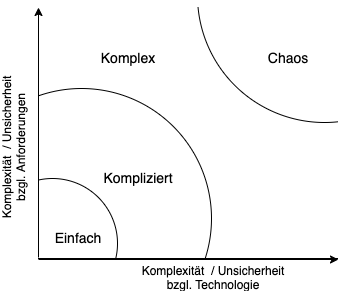
\includegraphics[scale=0.65	]{stacey.png}
	\caption[center]{Die Stacey Matrix angelehnt an \cite{stacey_img}}
	\label{fig:stacey}
\end{figure}

Eine Herausforderung zu beginn vieler Projekte stellt die Wahl einer passenden Projektmanagement Strategie da. Hierbei kann die Stacey Matrix \cite{Stacey2011StrategicMA} unterstützen, indem Projekte in Einfach, Kompliziert, Komplex oder Chaotisch klassifiziert werden (siehe Abbildung \ref{fig:stacey}). Die Klassifizierung wird anhand der Unklarheit und Komplexität der eingesetzten Technologien (Wie wird das Projekt umgesetzt), sowie der Klarheit über die Anforderungen an das Projekt (Was wird in dem Projekt umgesetzt) vorgenommen. Bei einer Klassifizierung im "oberen" komplizierten Bereich bis hin zum Chaotischen Bereich sollten Methoden aus dem Agilen Umfeld, in unserem Fall Kanban oder Scrum eingesetzt werden. Bei einer Klassifizierung als Einfach oder im unteren Komplizierten Bereich kann, muss aber nicht, auch das Wasserfallmodell verwendet werden.

\subsection{Besonderheiten in Data Science Projekten}\label{sec:1}

Bei der Durchführung von Data Science Projekten ist zu Projektstart oft nicht genau abzuschätzen, in wie fern die festgelegten Ziele erreicht werden können. Das liegt unter Anderem daran, dass die Auswahl der eingesetzten Technologien erst im laufe des Projektes stattfinden kann. Das liegt unter anderem daran, dass zu Beginn oft noch unklar ist, ob und wie gut die Ziele zu realisieren sind. Darüber hinaus herrscht oft Unklarheit über die wahre Qualität der zu verarbeitenden Daten. Diese wird in der Praxis eher über statt unterschätzt \cite{agile_pm}.

Durch die oben beschriebenen Unklarheiten bezüglich der Technologien sowie der Ziele sind die meisten Data Science Projekte in der Stacey Matrix eher ab der komplizierten Stufe einzuordnen.

\section{Einfluss von Persönlichkeiten auf das Projektmanagement}\label{sec:2}

\subsection{Persönlichkeiten nach DISG}
Nach dem DISG-Modell \cite{disc} lassen sich Persönlichkeiten in die Bereiche Dominant(D), Initiativ(I), Stetig(S) und Gewissenhaft(G) unterteilen. Eine Persönlichkeit setzt sich meist aus unterschiedlichen Bereichen verschieden stark ausgeprägt zusammen. Mit Hilfe eines DISG-Persönlichkeitstests kann ein Persönlichkeitsprofil erstellt werden. Typische Eigenschaften der verschiedenen Persönlichkeitstypen können der folgenden Auflistung entnommen werden.

\begin{description}[align=left]
	\item [Dominant] Entschlossen, willensstark, direkt, herausfordernd, ergebnisorientiert, selbstbewusst, durchsetzungsfähig, risikobereit
	\item [Initiativ] Optimistisch, kommunikativ, beeinflussend, enthusiastisch, emotional, anregend, spontan, gesellig, freundlich, unterhaltsam
	\item [Stetig] Loyal, hilfsbereit, geduldig, teamfähig, unterstützend, bescheiden, verbindlich, entspannt, zuverlässig, ausdauernd
	\item [Gewissenhaft] Hohe Maßstäbe, perfektionistisch, selbsdiszipliniert, vorsichtig, analytisch, gewissenhaft \cite{disg_charakteristika}
\end{description}

%Ideen: Sind Dominant und Initiativ ungeduldig?
%

\subsection{Auswirkung verschiedene Projektmanagement Methoden auf die DISG Persönlichkeiten}
Auss den oben beschriebenen Charaktereigenschaften der verschiedenen Persönlichkeitstypen nach dem DISG-Modell ergeben sich unterschiedliche stärken und schwächen. Im Folgenden werden typische Stärken und Schwächen der Charaktere beschrieben und dargelegt, wie verschiedene Projektmanagement Methoden oder Werkzeuge verwendet werden können, um den Schwächen entgegenzuwirken und die Stärken zu nutzen.

\subsection{Der Dominante}
Zu den größten Stärken des Dominanten gehört das Organisieren. Eine Organisation nach Kanban würde dem Dominanten den Raum geben, um Verbesserungen in der Organisation laufend einzubringen.

Zu den Schwächen gehört, dass durch den Organisations und Diskussionsdrang zu viele Details zu ausgiebig diskutiert werden. Somit ist vor allem wichtig, dass in Daily Standup Meetings die ausgemachten Redezeiten eingehalten werden. Da der Dominante gerne Autoritäten überschreitet ist es zu empfehlen, bei einem Modell nach Kanban einer dominanten Persönlichkeit nicht die Aufgabe für die Kommunikation mit den Stakeholdern zu überlassen. Des weiteren nimmt sich der Dominante gerne zu viel vor. Dies kann man entgegen wirken mit X und X.

Heruntergebrochen auf die 3 Projektmanagement Methoden würde sich der Dominante wohl in einem Projekt, dass nach Kanban organisiert wird, am wohlsten und in einem Wasserfall-Projekt am unwohlsten fühlen.

\subsection{Die Initiative}
Zu den größten Stärken der Stetigen gehört ihre Kreativität.

Die Kreativität würde bei einem Wasserfallmodell untergehen, wenn die 

\subsection{Der Stetige}
...

\subsection{Die Gewissenhafte}
Qualitätsbewusstsein
...


\subsection{Teamzusammensetzung}
Bei einem Team also mit überwiegend X und X blablabla.

\section{Beispiele}
Wenn noch Platz ist, könnten hier Beispiele aus der Praxis oder mit fiktiven Personas beschrieben werden.

\section{Fazit}
Hier ein Fazit.

\bibliographystyle{asmems4}

% Here's where you specify the bibliography database file.
% The full file name of the bibliography database for this
% article is asme2e.bib. The name for your database is up
% to you.
\bibliography{pm}

\end{document}
